\documentclass{hcmutarticle}

% gói để tạo chữ giả, xóa đi khi viết báo cáo
\usepackage{lipsum}

% create the header for this file
\fancyhead[RO, LE]{\bf Bài toán khai báo tài liệu trích dẫn}


\begin{document}
\thispagestyle{empty}
\begin{center}
\LARGE\bfseries ĐẠI HỌC QUỐC GIA TP HỒ CHÍ MINH \\
TRƯỜNG ĐẠI HỌC BÁCH KHOA
\end{center}

\begin{center}

\includegraphics[scale=0.2]{hcmut.pdf}\\[1cm]
\end{center}

\vspace{1cm}

\begin{center}
\Large \bfseries BÁO CÁO BÀI TẬP LỚN MÔN LẬP TRÌNH LOGIC VÀ RÀNG BUỘC\\[0.5cm]
\end{center}
\rule{\textwidth}{1pt}
\vspace{2pt}
\begin{center}
\Huge
\begin{tabular}{@{}l}
Study Min-Conflict Hill Climbing
\\and Min-Conflict Random Walk algorithms.
\\Try the algorithms on N-QUEENS problem\\[6pt]
\end{tabular}
\end{center}
\rule{\textwidth}{1pt}\\[1cm]

\vspace{2cm}

\begin{minipage}[t]{0.60\linewidth}
\textbf{GVHD}: \\
\ TS. Dương Tuấn Anh
\end{minipage}
\begin{minipage}[t]{0.40\linewidth}
\textbf{Sinh viên thực hiện:}\\
Nguyễn Quốc Long - MSSV:1770023
\end{minipage}

\vspace{3cm}

\begin{center}

\textbf{TP.Hồ Chí Minh},
20/07/2018.

\end{center}



\newpage

\tableofcontents 

\newpage

\title{Bài luận tìm hiểu giải thuật Min-conficts}

\author{  Nguyễn Quốc Long\inst{1}} 

\institute{ MSSV: 1770023}




\maketitle



\begin{abstract}
Tài liệu tìm hiểu về giải thật Min-coflicts


\end{abstract}

\begin{keywords}
algorithm, Min-coflicts algorithms, Min-Conflict Hill Climbing algorithms, Min-Conflict Random Walk algorithms ...
\end{keywords} 


\section{Giới thiệu}

\textbf{Thuật giải xung đột tối thiểu} 
 là một giải thuật dùng khá phổ biến trong giải hệ ràng buộc CSP. Thuật giải xuang đột tối thiểu sẽ chọn ngẫu nhiên một biến nào đó dính líu tới một ràng buộc bị vi phạm rồi chọn một trị từ miền trị của biến này sao cho tối thiểu hóa số lượng những vi phạm ràng buộc có thể xảy ra. Vì vậy thuật giải xung đột tối thiểu thuần túy có thể không thoát ra được điểm tối ưu cục bộ. Thuật giải thường kết hợp với chiến lược random-walk. Với môt biến nào đó được chọn, chiến lược bước ra ngẫu nhiên lấy ngẫu nhiên một trị từ miền trị của biến này với xác suất p, và áp dụng theo Thuật giải xung đột tối thiểu với xác suất 1-p. Giá trị của thông số p có ảnh hưởng lên hiệu quả của Thuật giải xung đột tối thiểu, thuật giải này được gọi là Min-conflict Random Walk.

\textbf{Thuật giải leo đồi (Hilll-climbing)}
 chính là nền tảng cơ sở của các ký thuật tìm kiếm cục bộ.Ở mỗi bước của việc tìm kiếm, chúng ta sẽ chọn một bước mà nó cải thiện giá trị hàm mục tiêu để thực hiện. Trong thuật giải leo đồi, chỉ những bước chuyển cải thiện được hàm chi phí hoặc không làm chi phí thay đổi thì mới đươc chọn vì vậy việc tìm kiếm sẽ liên tục bước lên vị trí cao hơn cho đến khi nó gặp điều kiện ngừng. Mặc dù đây là một giải thuật đơn giản nhưng lại hiệu quả  và rất mạnh trong việc giải quyết các bài toán CSP lớn.
%$- $  Sao chép các đoạn văn bản từ bài viết của người khác?\\



 Trong tài liệu này chúng sẽ giới thiệu cho các bạn giải thuật Min-conflic Hill Climbing and Min-Conflict Random Walk.
. Hy vọng tài liệu sẽ thực sự hữu ích cho các bạn.\\

\newpage

%%%%%%%%%%%%%%
\section{Tóm tắt nội dung}\label{survey}
Bài toán N-Queen problem đã là một bài toán kinh điển trong giới khoa học , nhất là giới khoa học máy tính. Trong bài tiểu luận này, tác giả sẽ phân tích bài toán N-Queen problem và giải quyết bài toán đó bằng thuật toán Min-Confilt Hill climbing và thuật toán Min-Conflict Random Walk.
Với thuật toán xung đột tối thiểu, \\

{\bfseries  Sau đây là cách trích dẫn tài liệu tham khảo theo quy định của Bộ Giáo Dục và Đào Tạo:}\\

Trong bài viết, bất cứ dẫn chứng nào cũng phải kèm tên tác giả và thời điểm công bố (xuất bản). Nếu tác giả người nước ngoài chỉ cần liệt kê HỌ. Nếu tài liệu chuyển ngữ sang tiếng Việt , cách dẫn chứng như trên.Nếu tác giả là người Việt hoặc tiếng nước ngoài thì liệu kê đầy đủ như chính tác giả đã viết.\\
Sau đây, chúng ta sẽ đi vào cụ thể từng chuẩn khai báo tài liệu trích dẫn.
%%%%%%%%%%%%%%
\section{Giới thiệu vấn đề }\label{dev}

\subsection{N-Queen problem}

Bài toán tám quân hậu là bài toán đặt tám quân hậu trên bàn cờ vua kích thước 8x8 sao cho không có quân hậu nào có thể "ăn" được quân hậu khác, hay nói khác đi không quân hậu nào có để di chuyển theo quy tắc cờ vua. Màu của các quân hậu không có ý nghĩa trong bài toán này. Như vậy, lời giải của bài toán là một cách xếp tám quân hậu trên bàn cờ sao cho không có hai quân nào đứng trên cùng hàng, hoặc cùng cột hoặc cùng đường chéo. Bài toán tám quân hậu có thể tổng quát hóa thành bài toán đặt n quân hậu trên bàn cờ nxn(n >= 4).


\begin{center}
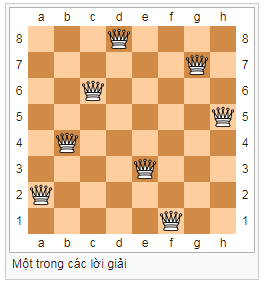
\includegraphics[scale=1]{image/hinhboard8x8}\\[1cm]
\end{center}

\subsubsection{Lịch sử}.
\\
Bài toán được đưa ra vào 1848 bởi kỳ thủ Max Bezzel, và sau đó nhiều nhà toán học, trong đó có Gauss và Georg Cantor, có các công trình về bài toán này và tổng quát nó thành bài toán xếp hậu. Các lời giải đầu tiên được đưa ra bởi Franz Nauck năm 1850. Nauck cũng đã tổng quát bài toán thành bài toán n quân hậu. Năm 1874, S. Gunther đưa ra phương pháp tìm lời giải bằng cách sử dụng định thức, và J.W.L. Glaisher hoàn chỉnh phương pháp này.

\subsubsection{Xây dựng một lời giải}.
\\
Có một giải thuật đơn giản tìm một lời giải cho bài toán n quân hậu với n = 1 hoặc n >= 4:\\
Chia n cho 12 lấy số dư r. (r= 8 với bài toán tám quân hậu).\\
Viết lần lượt các số chẵn từ 2 đến n.\\
Nếu số dư r là 3 hoặc 9, chuyển 2 xuống cuối danh sách.\\
Bổ sung lần lượt các số lẻ từ 1 đến n vào cuối danh sách, nhưng nếu r là 8, đổi chỗ từng cặp nghĩa là được 3, 1, 7, 5, 11, 9, ….\\
Nếu r = 2, đổi chỗ 1 và 3, sau đó chuyển 5 xuống cuối danh sách.\\
Nếu r = 3 hoặc 9, chuyển 1 và 3 xuống cuối danh sách.\\
Lấy danh sách trên làm danh sách chỉ số cột, ghép vào danh sách chỉ số dòng theo thứ tự tự nhiên ta được một lời giải của bài toán.\\
Sau đây là một số ví dụ: \\
$*$ 14 quân hậu (r = 2): 2, 4, 6, 8, 10, 12, 14, 3, 1, 7, 9, 11, 13, 5.\\
$*$ 15 quân hậu (r = 3): 4, 6, 8, 10, 12, 14, 2, 5, 7, 9, 11, 13, 15, 1, 3.\\
$*$ 20 quân hậu (r= 8): 2, 4, 6, 8, 10, 12, 14, 16, 18, 20, 3, 1, 7, 5, 11, 9, 15, 13, 19, 17.\\

\subsubsection{Số lời giải cho bài toán n quân hậu}.
\\
Ta có bảng sau đây cho n quân hậu
\begin{center}
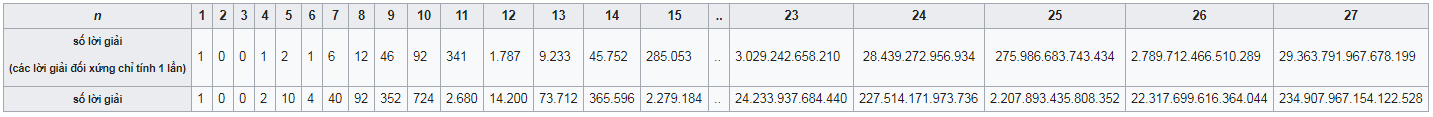
\includegraphics[scale=0.45]{image/n-board}\\[1cm]
\end{center}

\subsubsection{Giải thuật đệ quy và quay lui tìm kiếm tất cả các lời giải}.
\\
Trong giải thuật này, mỗi lời giải được ký hiệu bằng một mảng solution[1$..$n], trong đó solution[i]= j là cột mà quân hậu ở hàng thứ i đứng. Theo tính chất số học của các ô trên bàn cờ n x n, các ô trên các đường chéo cộng chứa ô (i, j) đều có tổng chỉ số hàng với chỉ số cột bằng i+j. Tổng này nhận các giá trị từ 2 đến 2n nên ta đánh số các đường chéo này từ 1 đến 2n-1. Như vậy các ô trên đường chéo cộng thứ nhất có tổng chỉ số dòng và cột là 2, các ô trên đường chéo thứ k có tổng ấy là k+1. Ta dùng một mảng Boolean Okplus[1..2n-1] để ký hiệu trạng thái đã có quân hậu nào trên đường chéo cộng thứ k chưa, nghĩa là Okplus[k]=True nếu đã có một quân hậu đứng chiếm giữ đường chéo cộng thứ k. Tương tự, các ô trên một đường chéo trừ có hiệu như nhau. Hiệu này nhận giá trị từ 1-n đến n- 1. Đánh số từ 1 đến 2n-1 từ đường chéo có hiệu chỉ số dòng trừ chỉ số cột là 1-n đến đường chéo có hiệu ấy bằng n-1. Khi đó đường chéo trừ thứ k có hiệu chỉ số dòng trừ chỉ số cột là k-n. Ta cũng dùng mảng okminus[1..2n-1] để chỉ trạng thái của các đường chéo này.

Giải thuật này cố gắng đặt quân hậu ở dòng thứ i vào cột nào đó, bắt đầu từ dòng thứ nhất (luôn có thể đặt được). Nếu ở dòng thứ i ta đặt quân hậu vào cột thứ j, thì nó khống chế tất cả các ô trong cột thứ j, đường chéo cộng thứ i+j-1, đường chéo trừ thứ i-j+n. Nếu có thể đặt được quân hậu ở dòng i và i = n ta có một lời giải. Nếu đặt được và i < n ta tiếp tục cố gắng đặt quân hậu tiếp theo vào dòng thứ i+1. Nếu không đặt được, ta quay lại nhấc quân hậu ở dòng thứ i-1 và tìm phương án tiếp theo của dòng thứ i-1.





























{\em Vào cuối của các thông tin được trích dẫn:}

fluoride nước cũng như các sản phẩm có chứa chất florua khác nhau như kem đánh răng cung cấp các ion florua cần thiết cho remineralization 1.

{\em Trong các thông tin được trích dẫn:}

Rakita 1 nói rằng nước có chất fluoride cũng như các sản phẩm có chứa chất florua khác nhau như kem đánh răng cung cấp các ion florua cần thiết cho remineralization.


\paragraph{Nghiêng số}.

{\em Vào cuối của các thông tin được trích dẫn:}

fluoride nước cũng như các sản phẩm có chứa chất florua khác nhau như kem đánh răng cung cấp các ion florua cần thiết cho remineralization ( {\itshape 1} ).

{\em Trong các thông tin trích dẫn:}

Rakita ( {\itshape 1} ) tuyên bố rằng nước có chất fluoride cũng như các sản phẩm có chứa chất florua khác nhau như kem đánh răng cung cấp các ion florua cần thiết cho remineralization.


\paragraph{Tên tác giả và năm xuất bản}.

{\em Vào cuối của các thông tin được trích dẫn:}

fluoride nước cũng như các sản phẩm có chứa chất florua khác nhau như kem đánh răng cung cấp các ion florua cần thiết cho remineralization (Rakita, 2004).

{\em Trong các thông tin trích dẫn:}

Rakita nước có chất fluoride cũng như các sản phẩm có chứa chất florua khác nhau như kem đánh răng cung cấp các ion florua cần thiết cho remineralization (2004).

\paragraph{Làm thế nào để định dạng danh sách tham khảo}.

{\bfseries Sách}

{\em Độc thân tác giả}

Chang, R. Tổng Hóa: Các khái niệm cần thiết, lần thứ 3, McGraw-Hill: Boston, năm 2003.

{\em Thay đổi nội dung sách}

Gbalint-Kurti, GG Wavepacket Lý thuyết của hình ảnh phân li và tán xạ phản ứng. 
{\em Sách trong Series}

Omega-3 axit béo: Hóa học, dinh dưỡng, Y tế và ảnh hưởng; Shahidi, F., Finley, JW, Eds; ACS Hội thảo Series 788; Hội Hóa học Mỹ: Washington, DC năm 2001.

{\em Điều từ một cuốn sách tham khảo}

Luyện kim bột. Kirk-Othmer Bách khoa toàn thư của Công nghệ hóa học, lần thứ 3; Wiley: New York, năm 1982, Vol. 19, Trang 28-62.

{\bfseries Các bài viết}

{\em Bài báo trong một tạp chí khoa học}

Evans, DA; Fitch, DM, Smith, TE; Cee, VJ Áp dụng các phản ứng nghịch đảo phức tạp để tổng hợp Phorboxazole B. J. Am. Chem. Sóc 2000, 122 , 10033-10046.

{\em Bài báo trong một tạp chí phổ biến / không khoa học}

Manning, R. Siêu hữu cơ, 2004, pp 176-181.

{\em Điều từ một tạp chí trực tuyến}

Peacock-Lopez, E. Chính xác giải pháp tiềm năng Quantum. 2007, 11 , 383-393 http://chemeducator.org/bibs/0011006/11060380lb.htm 

{\bfseries Luận án, Bằng sáng chế, Hội nghị, Báo cáo kỹ thuật}

{\em Đề tài}

Thoman, JW, Jr nghiên cứu của vô hiệu hóa một phân tử hoạt động bề mặt -Tiến sĩ Luận án, Viện Công nghệ Massachusetts, Cambridge, MA, 1987.
hoăc

Gehring, A. Tiến sĩ. Luận văn, Đại học Harvard năm 1998.

{\em Bằng sáng chế}

 Phát hiện, cách ly, Thanh lọc độc tố Clostridiu, ngày 24 tháng 3 1992.

{\em Hội nghị / Hội nghị (toàn văn)}

Winstein, Trong Giáo dục Đại học Hóa chất, Kỷ yếu của Hội nghị Quốc tế về Giáo dục Đại học Hóa chất, Frascati (Rome), Italy, 16-19 tháng Mười, năm 1969; Chisman, DG. Ed; Butterworths: London, 1970.

{\em Hội nghị / cuộc họp }

Kaplan, LJ; Selder, A. sách tóm tắt, 213th ACS Hội nghị Quốc gia, San Francisco, CA, 13-ngày 17 tháng tư, năm 1997, Hội Hóa học Mỹ: Washington, DC, năm 1997, CHED-824.

{\em Báo cáo kỹ thuật }

Crampton, SB; McAllaster, hiệu ứng chuyển động trung bình trong maser nguyên tử Hydrogen đông lạnh, WMC-AFOSR-002; NTIS: Springfield, VA, 1983.

{\bfseries Web / Mạng}

Lưu ý: trình duyệt web khác nhau phá vỡ các văn bản ở những nơi khác nhau của một URL. URL nên bắt đầu trên cùng một dòng như phần còn lại của các thông tin trích dẫn, với một đoạn chèn vào sau khi một dấu gạch chéo, nếu cần thiết.

{\em Trang web}

National Library of Medicine. Y tế và môi trường Độc Chất: Dịch vụ Thông tin chuyên ngành. http://sis.nlm.nih.gov/enviro.html (truy cập ngày 23 tháng 8 2004.

{\em Điều từ một tạp chí trực tuyến}

Peacock-Lopez, E. Chính xác Giải pháp tiềm năng Quantum. Chem. Ed. 2007, 11 , 383-393 http://chemeducator.org/bibs/0011006/11060380lb.htm (truy cập ngày 23 tháng 8 năm 2007).

{\em Điều từ cơ sở dữ liệu văn bản đầy đủ}

Begley, S. Khi não của bạn ngừng hoạt động Newsweek [Online] ngày 02 Tháng Bảy 2007, 62 p. Mở rộng. http:/galegroup.com (truy cập ngày 23 tháng 8 năm 2007).



\subsection{Min-Conflict}

{\em AMA Manual of Style}: Hướng dẫn dành cho Tác giả và biên tập viên là một hướng dẫn phong cách bởi các biên tập viên của JAMA (Tạp chí của Hiệp hội Y khoa Mỹ) và tạp chí - gần đây nhất xuất bản Oxford University Press [ 1 ] [ 2 ] . Quy định cụ thể bằng văn bản và trích dẫn phong cách cho sử dụng trong các ấn phẩm học thuật trong y học quốc tế, bao gồm cả JAMA và tạp chí - . Nó được xuất bản lần đầu vào năm 1962, và phiên bản hiện tại của nó, 10, ra đến năm 2007 [ 1 ] . Hướng dẫn AMA của phong cách bao gồm một bề rộng chủ đề cho tác giả và biên tập viên trong y học và các lĩnh vực liên quan đến sức khỏe và bao gồm 25 chương:{\em Phần 1. Chuẩn bị Điều Xuất bản - 1 loại điều, 2 Chuẩn bị bản thảo, 3 Tham khảo 4 Visual trình bày dữ liệu, 5 Xem xét đạo đức và pháp lý, 6 biên tập đánh giá và chế biến; Mục 2. (US) - 7. Ngữ pháp, 8. Dấu chấm câu, 9. Số nhiều, 10. Hoa, 11. Chính xác và ưu tiên sử dụng, 12. Không phải tiếng Anh từ, cụm từ, và nhãn hiệu Accent, 13. Chỉ số y tế; Phần 3. Thuật ngữ - 14. Chữ viết tắt, 15. Danh mục này, 16. Eponyms, 17. Hy Lạp Thư Mục 4. Đo lường và định lượng 18. Các đơn vị đo lường, 19. Số và Tỷ lệ phần trăm, 20.Thiết kế nghiên cứu và thống kê, 21. Thành phần toán học; Mục 5. Thông tin kỹ thuật - 22. Kiểu chữ, 23. Chỉnh sửa bản thảo và Soát lỗi, 24.Glossary Số Publishing, 25. Tài nguyên.}
\subsubsection{Min-Conflict Hill Climbing algorithm}.

Tham khảo thông tin sử dụng được thực hiện trong danh sách tham khảo. Điều này bao gồm nhưng không phải là giới hạn các bài báo được công bố hoặc được chấp nhận cho công bố trong in ấn hàng loạt nghiên cứu hoặc lưu thông hoặc tạp chí điện tử, tạp chí, báo, cuốn sách đã được công bố, chấp nhận cho xuất bản, giấy tờ trình bày tại các cuộc họp chuyên nghiệp, tóm tắt, đề tài, CD-ROM, bộ phim, băng hình, và audiofiles, chèn gói hoặc tài liệu hướng dẫn của nhà sản xuất, chuyên khảo; chính thức báo cáo, cơ sở dữ liệu và các trang web, trường hợp pháp luật; bằng sáng chế, và phiên bản mới. Danh sách tham khảo Tài liệu tham khảo cần được liệt kê theo số thứ tự ở phần cuối của bản thảo (trừ trường hợp quy định tại mục 3.3 và 3.5 trong {\itshape Hướng dẫn US AMA}). Hai tài liệu tham khảo không nên kết hợp theo một số tham chiếu duy nhất.

\subsubsection{Min-Conflict Random Walk algorithm}.


Trích dẫn trong ngoặc trong các văn bản của tài liệu tham khảo đáp ứng các tiêu chuẩn để đưa vào danh sách tài liệu tham khảo nên được giới hạn trường hợp trong danh sách tham khảo sẽ không được sử dụng, tin bài cáo phó. Lưu ý rằng trong các văn bản :

Tài liệu tham khảo trong văn bản Tác giả 

• Có thể không được đặt tên 

• Tiêu đề này có thể không được 

• Tên của tạp chí là viết tắt chỉ khi kèm theo trong ngoặc đơn

 • số trang hòa nhập được 
 
Một số nguồn lực, chẳng hạn như URL Web, có thể được liệt kê trong văn bản khi nó là trang Web chính nó được gọi chứ không phải là nội dung trên trang web đó.

{\bfseries Ví dụ}

Wiese gần đây đã báo cáo rằng chất chiết xuất từ quả của cây xương rồng lê gai có vừa phải có hiệu lực vào việc giảm các triệu chứng nôn nao rượu ({\itshape Arch Intern} Med. 2004; 164 [12] :1334-1340). 

Các tác dụng của chiết xuất từ quả của cây xương rồng lê gai vào việc giảm Các triệu chứng của say rượu cồn đã được báo cáo trong một vấn đề gần đây của tài liệu lưu trữ {\itshape Nội khoa} (2004, 164 [12] :1334-1340). 

{\itshape Archives of Internal Medicine} bài viết (2004, 164 [12] :1334-1340) về tác động của một trích xuất trái cây của cây xương rồng lê gai làm giảm các triệu chứng của rượu nôn nao nhận được công khai rộng rãi (ví dụ, USA Today ngày 29 tháng 6, 2004:7 D)



%%%%%%%%%%%%%%
\section{Kết Luận }\label{result}
Tài liệu được thực hiện  với sự giúp đỡ tận tình của giáo viên hướng dẫn, Thầy TS. Dương Tuấn Anh\\
Trong quá trình nghiên cứu, thực hiện không thể tránh khỏi những  thiếu sót, kính mong quý thầy  cô và các bạn đóng góp thêm để tài liệu thêm hoàn thiện.\\
Xin chân thành cảm ơn.




%%%%%%%%%%%%%%
\section{Tài liệu Tham Khảo }




%%%%%%%%%%%%%%%%%%%%%%%%%%%%%%%%%

http://en.wikipedia.org\\
http://globaledu.com.vn/Thong-Tin-Chi-Tiet/1881/1881\\
http://library.williams.edu/citing/styles/acs.php\\

%%%%%%%%%%%%%%

\end{document}



